\chapter{Discrete physics-informed training for projection-based reduced-order models with neural networks (Article 3)}
\label{chap:article3}

\section*{Preface}

This chapter reproduces the peer-reviewed article \textit{``Discrete Physics-Informed Training for Projection-Based Reduced-Order Models with Neural Networks''} published in \textit{Axioms}~\cite{sibuet2025discrete}. Building directly on the PROM-ANN latent-space closure framework discussed in earlier chapters, this work addresses one of its main limitations: the lack of physics consistency during training when purely data-driven loss functions are used.

Specifically, this contribution introduces a discrete physics-informed training strategy that augments the standard snapshot reconstruction loss with an additional residual-based term derived directly from the finite element discretization of the governing equations. This dual-loss formulation drives the nonlinear manifold learned by the PROM-ANN to align not only with the snapshot data but also with the residual behavior that is minimized during the intrusive online projection. While the methodology is demonstrated here in the context of PROM-ANN, the same discrete residual-based loss could be integrated into other neural-network-based nonlinear manifold models, including convolutional autoencoders such as those proposed by Lee and Carlberg~\cite{lee2020model}, Romor et al.~\cite{romor2023non}, and Fresca and Manzoni~\cite{FRESCA2022114181}.

The approach is formulated to be general and not tailored exclusively to structural problems, making it relevant for a broad class of nonlinear systems. The methodology is demonstrated on a nonlinear hyperelastic cantilever benchmark under multi-axial loading, providing an alternative test case that complements convection-dominated examples such as the Burgers equation. This setting highlights how discrete physics-informed training can potentially improve residual fidelity and help close the gap between reconstruction error and true online solve error, especially in strongly nonlinear regimes.

\vspace{0.5em}
\noindent
The core idea can be summarized by the following schematic formulation:
\begin{equation}
\tilde{\mathbf{u}} = D_u(\mathbf{q}) = \mathbf{u}_{\text{ref}} + \boldsymbol{\Phi} \mathbf{q} + \overline{\boldsymbol{\Phi}}\, \mathcal{N}(\mathbf{q}),
\quad
\mathcal{L} = 
\underbrace{\mathcal{L}_\text{d}}_{\substack{\text{data-driven} \\ \text{reconstruction}}}
+ 
\underbrace{\mathcal{L}_\mathbf{R}}_{\substack{\text{discrete} \\ \text{residual consistency}}},
\label{eq:high_level_loss_preface}
\end{equation}

where \(\mathcal{N}(\mathbf{q})\) is the neural network closure and the total training loss combines reconstruction and discrete residual terms, promoting consistency between the learned manifold and the full-order residual behavior.


The paper details:
\begin{itemize}
    \item A rigorous derivation of the residual-based loss term, its normalization, and its integration into the PROM-ANN training workflow.
    \item An efficient coupling strategy between the physics solver (Kratos Multiphysics) and the neural network framework, including practical residual vectorization and Jacobian operations.
    \item A systematic numerical assessment illustrating the possibility of improving residual representation through discrete physics-informed training for intrusive nonlinear ROMs.
\end{itemize}

Overall, this chapter situates discrete physics-informed training as a meaningful step toward more robust and physically consistent nonlinear PROMs. Together with the kernel-based latent-space closure strategies presented in Chapter~\ref{chap:article4}, it forms a key component of this thesis’s broader contribution: bridging the gap between data-driven manifold learning and the residual-consistent projection frameworks needed for scalable applications.

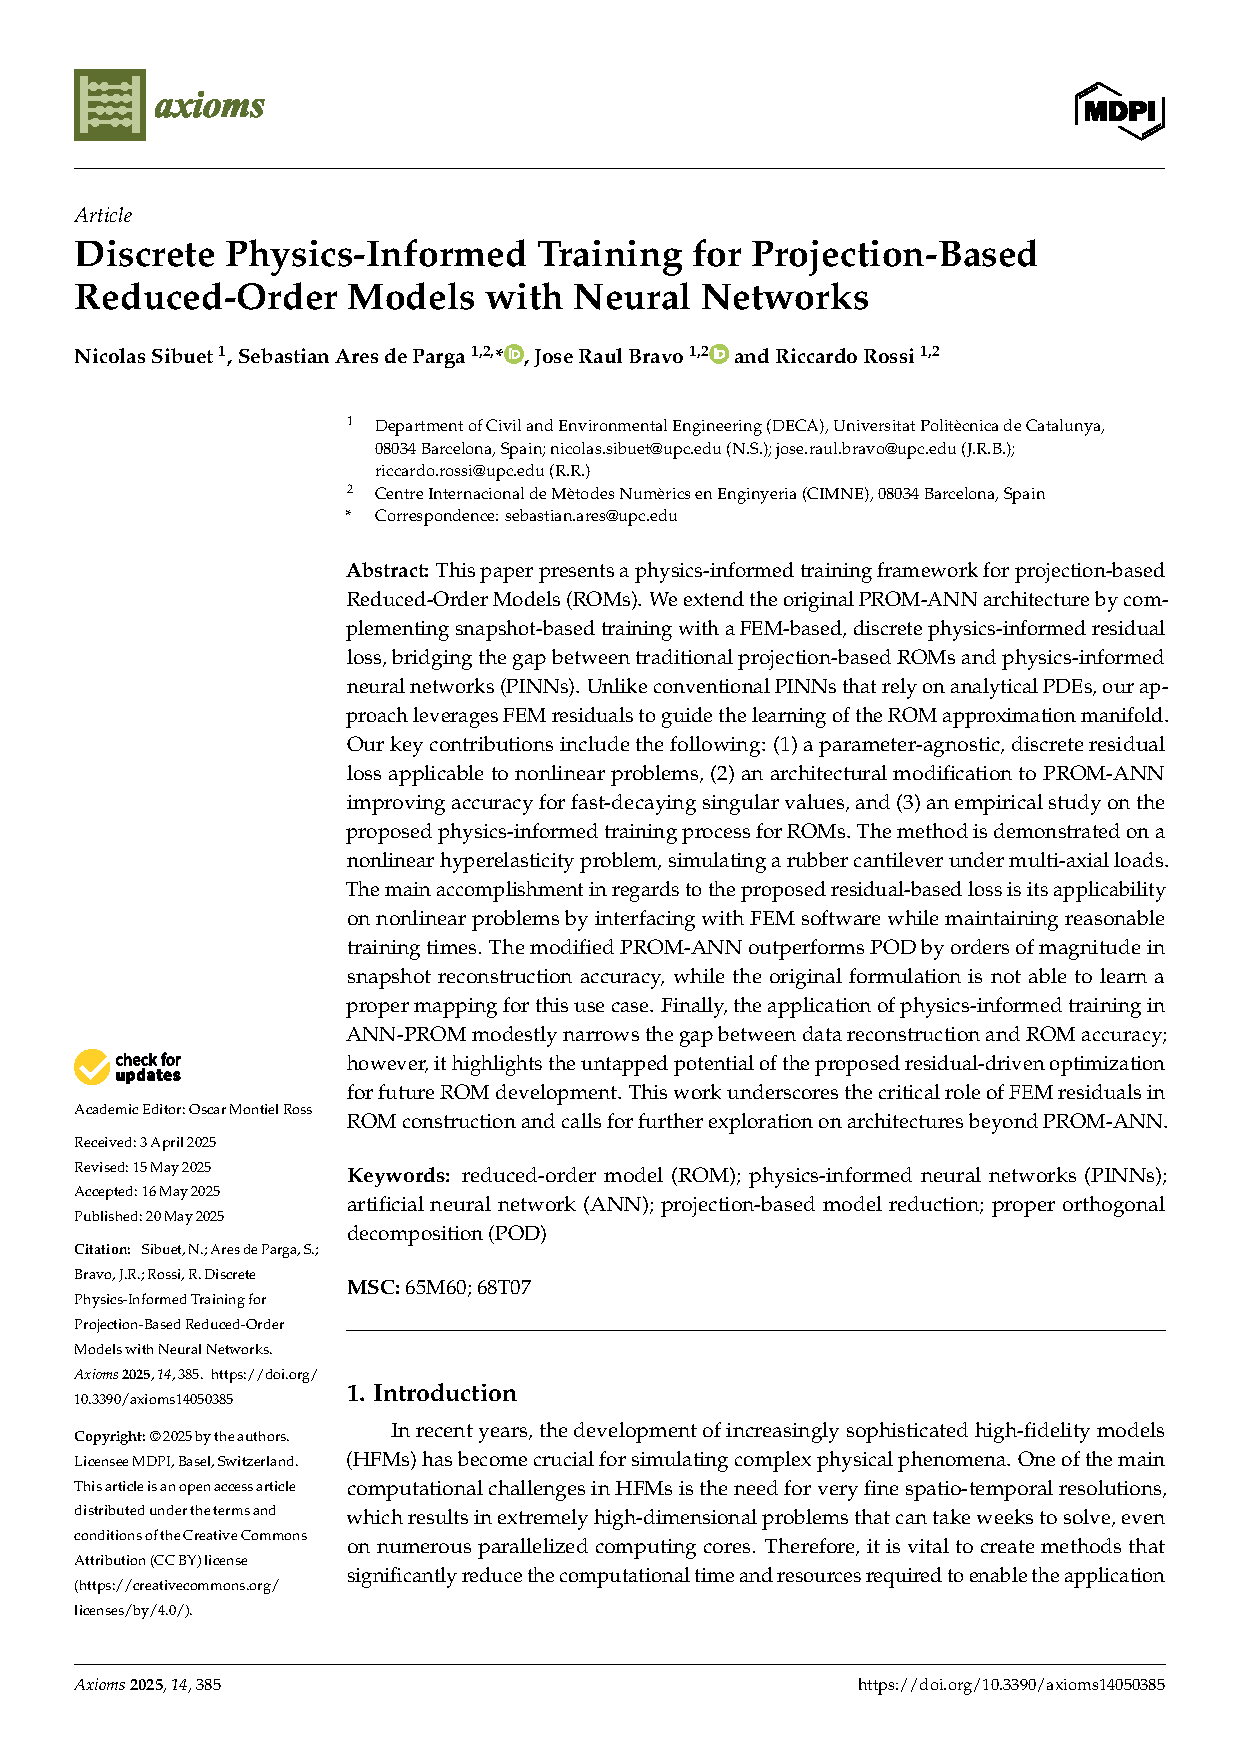
\includepdf[
  pages=-,
  pagecommand={},
  scale=0.92,
  delta=0 0,
  offset=32pt 0pt,
  turn=false
]{Papers/Discrete_Physics-Informed_Training_for_Projection-Based_Reduced-Order_Models_with_Neural_Networks.pdf}
